
\documentclass{article}
\usepackage{amsmath, xcolor, tikz, pgfplots, array, bm, tcolorbox, sfmath, enumerate}
\renewcommand{\familydefault}{\sfdefault}
\usepackage[top=0.5in, bottom=0.5in, left=1.25in, right=1.25in]{geometry}
\pagestyle{empty}
\raggedright


\pgfplotsset{compat = newest}
\usetikzlibrary{arrows.meta, calc, decorations.pathreplacing}
\pgfplotsset{every axis/.append style = {axis lines = middle}}
\pgfplotsset{every tick label/.append style={font=\scriptsize}}
\everymath{\displaystyle}

\newcounter{example}[section]
\newenvironment{example}[1][]{\refstepcounter{example}\par\medskip
   {\color{red}\textbf{Example~\theexample. #1}}}{\medskip}

\begin{document}

\section*{Exponential Functions}

\begin{tcolorbox}[colframe=orange!70!white, coltitle=black, title=\textbf{Summary}]
\begin{enumerate}
    \item Exponential functions are in the form $f(x) = b^x$, where $b>0$ and $b\neq 1$.
    \item The value of $b$ determines if the function is exponential growth or exponential decay.
    \item Exponential functions will have a horizontal asymptote in one direction.
    \item A special base is base $e \approx 2.718282$.
\end{enumerate}
\end{tcolorbox}
\vspace{0.5in}

\begin{tcolorbox}[colframe=green!60!black, title=\textbf{Exponential Function}]
An \textbf{exponential function} is a function in which each successive output value is obtained by {\color{violet}\textbf{multiplying}} the previous one by a constant value.
\end{tcolorbox}
\vfill

One example of an exponential function is the {\color{blue}\textbf{doubling function}}
\[ f(x) = 2^x \]
\vspace{0.25in}

\begin{minipage}{0.4\textwidth}
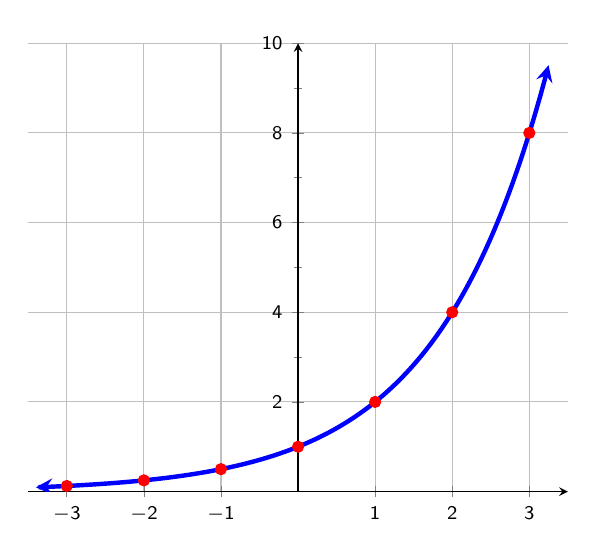
\begin{tikzpicture}
\begin{axis}[
xmin = -3.5, xmax = 3.5,
ymin = 0, ymax = 10, grid, minor y tick num=1
]
\addplot[color=blue, ultra thick, samples=200, smooth, domain=-3.4:3.25, <->, >=stealth] {2^x};
\addplot[color=red, mark = *, only marks] coordinates {(-3,0.125) (-2,0.25) (-1,0.5) (0,1) (1,2) (2,4) (3,8)};
\end{axis}
\end{tikzpicture}
\end{minipage}
\hspace{1cm}
\begin{minipage}{0.25\textwidth}
\setlength{\extrarowheight}{5pt}
\begin{tabular}{c|c}
    $x$ & $f(x)$ \\ \hline 
    $-3$ & $\tfrac{1}{8}$ \\[5pt]
    $-2$ & $\tfrac{1}{4}$ \\[5pt]
    $-1$ & $\tfrac{1}{2}$ \\[5pt]
    0   &   1   \\[5pt]
    1   &   2   \\[5pt]
    2   &   4   \\[5pt]
    3   &   8   
\end{tabular}
\end{minipage}
\vspace{0.5in}

As the values of $x \to -\infty$, \quad
$ 2^{\text{very big negative number}} \to 0 $   \newline\\
For instance,
$2^{-50} \approx 0.0000000000000008882$
\vspace{0.5in}

As the values of $x \to \infty$, \quad
$2^{\text{very big positive number}} \to \infty $   \newline\\ 
For instance,
$2^{50} = 1,125,899,906,842,624$
\vfill

\newpage

A function in the form $f(x) = b^x$ where $b$ is a fixed real number, $b > 0, b \neq 1$ is called an \textbf{exponential function of base $\bm{b}$}  \vspace{0.5in}

\begin{minipage}{0.35\textwidth}
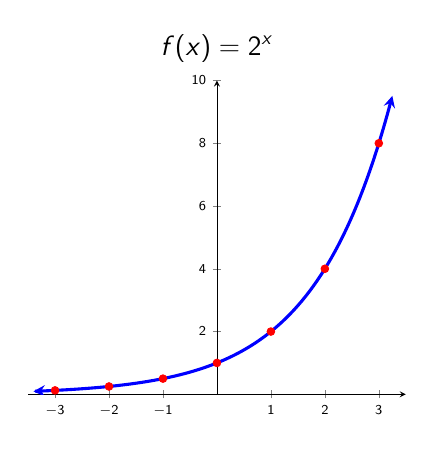
\begin{tikzpicture}[scale=0.7]
\begin{axis}[
xmin = -3.5, xmax = 3.5,
ymin = 0, ymax = 10,
title = {\Large $f(x)=2^x$}
]
\addplot[color=blue, ultra thick, samples=200, smooth, domain=-3.4:3.25, <->, >=stealth] {2^x};
\addplot[color=red, mark = *, only marks] coordinates {(-3,0.125) (-2,0.25) (-1,0.5) (0,1) (1,2) (2,4) (3,8)};
\end{axis}
\end{tikzpicture}
\end{minipage}
\hspace{0.5cm}
\begin{minipage}{0.45\textwidth}
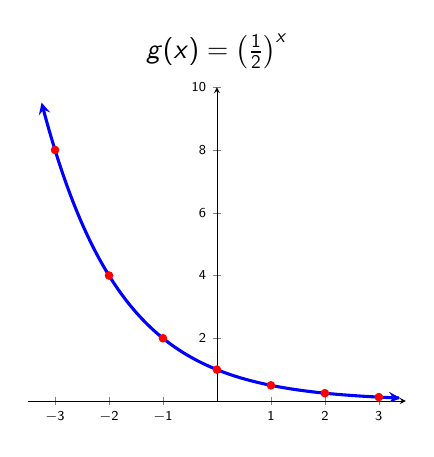
\begin{tikzpicture}[scale=0.7]
\begin{axis}[
xmin = -3.5, xmax = 3.5,
ymin = 0, ymax = 10,
title = {\Large $g(x) = \left(\frac{1}{2}\right)^x$}
]
\addplot[color=blue, ultra thick, samples=200, smooth, domain=-3.25:3.4, <->, >=stealth] {2^-x};
\addplot[color=red, mark = *, only marks] coordinates {(-3,8) (-2,4) (-1,2) (0,1) (1,0.5) (2,0.25) (3,0.125)};
\end{axis}
\end{tikzpicture}
\end{minipage}
\vspace{1in}

\subsection*{Properties of Exponential Functions}
For $f(x) = b^x$:   \newline\\
\begin{itemize}
    \item Domain is $(-\infty, \infty)$ and the range is $(0,\infty)$ \newline\\
    \item $(0,1)$ is on the graph of $f$ and $y=0$ is a horizontal asymptote. \newline\\
    % \item $f$ is one-to-one (has an inverse), continuous, and smooth.
\end{itemize}
\newpage


% For $f(x) = b^x$ when $b > 1$:  \newline\\
% \begin{itemize}
%     \item $f$ is always increasing  \newline\\  
%     \item $\lim_{x\to -\infty} = 0 \quad \text{and} \quad \lim_{x\to \infty} = \infty$ \newline\\ 
%     \item The graph of $f$ resembles
% \end{itemize}
% \begin{center}
%     \begin{tikzpicture}[scale=0.7]
%     \begin{axis}[
%     xmin = -2, xmax = 2,
%     ymin = 0, ymax = 4.5,
%     ticks=none
%     ]
%     \addplot[blue, very thick, samples=200, smooth] {2^x};
%     \end{axis}
%     \end{tikzpicture}
% \end{center}
% \vfill

% For $f(x) = b^x$ when $0 < b < 1$:  \newline\\
% \begin{itemize}
%     \item $f$ is always decreasing  \newline\\  
%     \item $\lim_{x\to -\infty} = \infty \quad \text{and} \quad \lim_{x\to \infty} = 0$ \newline\\ 
%     \item The graph of $f$ resembles
% \end{itemize}
% \begin{center}
%     \begin{tikzpicture}[scale=0.7]
%     \begin{axis}[
%     xmin = -2, xmax = 2,
%     ymin = 0, ymax = 4.5,
%     ticks=none
%     ]
%     \addplot[blue, very thick, samples=200, smooth] {2^-x};
%     \end{axis}
%     \end{tikzpicture}
% \end{center}
% \vfill

% \newpage 

% \begin{example}
% For each of the following,
% \begin{itemize}
%     \item Determine the end behavior of the parent function, $f(x)$.
%     \item Determine the transformations done to $f(x)$ to obtain $g(x)$. Be specific.
%     \item Determine the end behavior of $g(x)$.
% \end{itemize}
% \bigskip 
% \begin{enumerate}[(a)]
%     \item $f(x) = 3^x$; \quad $g(x) = 3^{5x+2} - 1$ \vfill 
%     \item $f(x) = (1.5)^x; \quad g(x) = -\frac{1}{4}\left(1.5\right)^{x} + 2$   \vfill 
%     \item $f(x) = \left(\frac{2}{3}\right)^x; \quad g(x) = \left(\frac{2}{3}\right)^{-x-5}$    \vfill 
% \end{enumerate}
% \end{example}

% \newpage 


\begin{example}
The value of a car can be modeled by $V(x) = 25\left(\frac{4}{5}\right)^x$, where $x \geq 0$ is the age of the car in years and $V(x)$ is the value in thousands of dollars.    \newline\\
\begin{enumerate}[(a)]
\item Find and interpret $V(0)$   \vfill

% \item Find the parent function and describe the function $V(x) = 25\left(\frac{4}{5}\right)^x$ using transformations.    \vfill

\item Find and interpret the horizontal asymptote of the graph of $V(x)$. \vfill
\end{enumerate}
\end{example}

\subsection*{Interest}

\subsubsection*{Simple Interest, $I$} 

\begin{itemize}
    \item Paid out at \emph{one moment in time}.
    \item $P$ dollars deposited into an account
    \item Interest rate $r$ (convert percent to decimal)
    \item Time $t$
\end{itemize}

\begin{align*}
    \text{Interest} &= \text{Principal} \cdot \text{rate} \cdot \text{time} \\
    I &= Prt
\end{align*}

\subsubsection*{Compound Interest, $A$}

\begin{itemize}
    \item Paid out on a \emph{regular basis}.
    \item $k$ times per year
\end{itemize}

\[
A = P\left(1 + \frac{r}{k}\right)^{kt}
\]

\newpage 

\begin{example}
Suppose \$20,000 is deposited into a retirement account that yields an interest rate of 6.5\% compounded quarterly. 
\begin{enumerate}[(a)]
    \item How much will be in the account after 3 years?  \vspace{1.25in}
    \item How much total interest was earned after 3 years?  \vspace{1.25in}
    \item How much will be in the account after 40 years?  \vspace{1.25in}
\end{enumerate}
\end{example}


\subsection*{Special Base $e$}

Of all possible bases for exponential functions, \\
the most common is the irrational base $e$ (\textbf{natural base}). \vspace{0.5in}

\begin{example}
Evaluate $f(x) = \left(1 + \frac{1}{x}\right)^x$ for very large values of $x$.
\end{example}
\vfill 

The {\color{blue}\textbf{exponential function}} has the form
\[
f(x) = a \cdot e^{bx}
\]
where $a$ and $b$ are real numbers.
\vspace{0.5in} 
\newpage 

\subsubsection*{Continuous Compounded Interest}
\vspace{0.25in}

\begin{itemize}
    \item Limits the amount of interest earned through compounding.
    \item Called \textit{continuous compounded interest}
    \item $A = Pe^{rt}$
\end{itemize}
\vspace{1.25in}

\begin{example}
This time \$20,000 is deposited at 6.5\% compounded continuously.
\begin{enumerate}[(a)]
    \item How much will be in the account after 3 years?  \vspace{1.5in}
    \item How much total interest was earned after 3 years?  \vspace{1.5in}
    \item How much will be in the account after 40 years?  \vspace{1.5in}
    \item What is the average rate of change from 3 to 40 years?
\end{enumerate}
\end{example}

\end{document}

